\renewcommand\thesection{\Alph{section}}

\begin{center} \textbf{PROJECT NARRATIVE} \end{center}

\section{Background}

%\subsection*{Fish passage in Washington state}

Migratory anadromous salmon and steelhead native to Western Washington (\textit{Oncorhynchus} spp.) rely on access to streams throughout their spawning and rearing phases of their complex life cycles. Barriers to fish passage, particularly poorly-designed culverts at road crossings, prevent fish from accessing potential habitat, hampering recovery efforts for declining populations. Reconnecting isolated habitat by correcting these culverts has been long identified as a crucial stage in watershed restoration \citep{roni_review_2002}. However, until fairly recently, barrier correction efforts have been limited by lack of available funds and political will. 
%NWIFC State of our Watersheds http://files.nwifc.org/sow/2020/state-of-our-watersheds-sow-2020-final-web.pdf
% Roni, Philip, Timothy J. Beechie, Robert E. Bilby, Frank E. Leonetti, Michael M. Pollock, and George R. Pess. “A Review of Stream Restoration Techniques and a Hierarchical Strategy for Prioritizing Restoration in Pacific Northwest Watersheds.” North American Journal of Fisheries Management 22, no. 1 (2002): 1–20. https://doi.org/10.1577/1548-8675(2002)022<0001:AROSRT>2.0.CO;2.

In 2001, Washington state was sued by the United States Department of Justice on behalf of 21 Northwest tribes for violating treaty fishing rights. The plaintiffs argued that state-owned culverts restrict salmon and steelhead access to historical upstream spawning habitat, leading to declines in salmon abundance and violating the Stevens Treaties which guarantee a right to fish within usual and accustomed fishing areas \citep{hickey_highway_2018}. The lawsuit, focused on Western Washington, hereafter the ``Case Area'', resulted in a 2013 federal court injunction requiring the State remove barrier culverts under its jurisdiction such that 90\% of blocked fish habitat is made accessible by 2030. The ruling mandates that the remainder of state-owned barrier culverts in the Case Area be restored for fish passage at the end of their life. The defendants filed an appeal, but after nearly two decades of legal battles, in 2018, the U.S. Supreme Court ruled in favor of the Tribes, upholding the 2013 federal injunction, ushering in a new era of fish passage policy in Western Washington. 


As of 2020, the Washington State Department of Transportation (WSDOT), responsible for the vast majority of state-owned culverts within the Case Area, has corrected 87 injunction barrier culverts opening up an estimated 383.3 miles of habitat at a cost of over \$159 million. Since the ruling, WSDOT has replaced an average of 12.4 culverts per year, including 13 in 2020. To satisfy the federal injunction, the rate of culvert replacements must ramp up dramatically. 
% Cite WSDOT annual report in this paragraph https://wsdot.wa.gov/sites/default/files/2019/09/20/Env-StrRest-FishPassageAnnualReport.pdf


\begin{wrapfigure}{r}{10cm}
\includegraphics[width=10cm]{figures/fig_mapconcrete.png}
\caption{Barriers to fish passage in the WDFW Fish Passage and Diversion Screening Inventory database by ownership type. (A) shows the entire Case Area (red dotted line) and (B) shows the diversity of barrier ownership entities in the Concrete, WA area along the Skagit River. Solid red box in (A) shows the extent of (B). Dark red lines show roads (data source: OpenStreetMap) and light blue lines show rivers, streams and other water bodies (data source: National Hydrology Dataset High Resolution).\label{fig:barrierMap}}
\end{wrapfigure}%

Importantly, the 2013 injunction strictly applies to state-owned culverts, whereas there exist an estimated 3,000 and 1,300 additional barrier culverts owned by counties and cities respectively, along with barrier culverts on private lands, often on the same streams as state-owned culverts \citep{brown_coming_2019}. Figure~\ref{fig:barrierMap} shows culvert barriers to fish passage recorded in the Washington Department of Fish and Wildlife (WDFW) Fish Passage and Diversion Screening Inventory (FPDSI) database, for all of the Washington Case Area (panel A) and along the Skagit River near Concrete, WA (panel B) as an example of a watershed where barriers owned by several entities exist. Specifically, for this portion of the Skagit River, 5 of 6 ownership entity types are indicated (cities, counties, federal, private, state, and other), demonstrating the complexity in salmon restoration in Washington State. The presence of multiple barrier ownership entities within a single watershed means that the benefits of any one entity's culvert restoration actions depend on the culvert restoration actions of other actors, suggesting potential gains from coordination. 

While non-state entities are not subject to the 2013 injunction, counties and cities across the region are ramping up their own barrier correction efforts in order to capitalize on the opportunity to restore habitat access throughout the Case Area \citep{brown_coming_2019}. However, counties and other actors are largely acting independently and there are differences between and within these ownership types in terms of goals, priorities, and resources for removing barriers to fish passage. For example, some counties conduct full habitat surveys in determining which barrier culverts to replace first, while others rely on GIS-based proxies. With regards to funding, while some cities and counties are able to access direct financial resources for fish passage projects, e.g.\ King County has used the surface water management fee to fund culvert restoration projects, other cities and counties do not have access to dedicated funding streams, primarily relying on grant funding.  

Fish passage restoration efforts in Washington state are not entirely uncoordinated. The Brian Abbott Fish Barrier Removal Board was established by the Washington State Legislature in 2014 to recommend priority projects to the Governor's Office and Legislature for funding, thereby promoting the coordinated and strategic removal of barriers to fish passage. In the 2021-2023 biennium, 87 ranked projects were recommended for funding at a total of \$61.3 million. Grant applicants include cities, counties, and non-profit organizations. There is demand from both the Legislature and grantees to better define the Board's selection criteria for potential projects and overall prioritization strategy. 

%\subsection*{Tailoring optimization for Washington fish passage prioritization}

There is a rich academic literature applying optimization tools to fish passage \citep{ohanley_optimizing_2005, kuby_multiobjective_2005, couto_safeguarding_2021}, i.e.\ researchers have developed robust methods for identifying restoration plans (combinations of barriers to correct) that maximize the return on investment for a given budget. Recently these tools have gained traction with resource managers. Examples include  \href{https://fishpass.psmfc.org}{FISH\emph{Pass}}, adopted by the California Fish Passage Forum in 2019, and \href{https://greatlakesconnectivity.org}{FishWerks} developed for the Great Lakes region as a collaboration between Cornell University and the University of Wisconsin. 

Our proposed research will develop a data-driven optimization framework for project prioritization, within the Case Area of Washington State, that synthesizes multiple geospatial datasets with statistical economic and ecological models to identify fish passage restoration plans that maximize ecological, social, and economic objectives at a given funding level. Our project will draw on relevant features and methods from the rich literature in fish prioritization and from lessons learned from the rollout of FISH\emph{Pass} in California (see Letter of Support from Bob Pagliuco contributor to FISH\emph{Pass}).

With our framework, we will assess the tradeoffs between key management objectives (e.g.\ increasing salmon habitat, ensuring an equitable distribution of habitat gains across user groups, and mitigating investment risks), gains from coordinating barrier culvert replacement across key actors (e.g.\ the state, counties, and cities), and gains from alternative funding streams (e.g.\ allocating large sums of money upfront versus allocating those same dollars slowly over time). We will also use our framework to assess path dependency, i.e.\ how optimal barrier removal projects are determined by past actions, and explore how optimal barrier removal plans change when conditioned on assumed actions of key players (e.g.\ assuming all state-owned barriers are corrected by 2030).

%While previous work has identified efficiency gains from coordinating barrier correction across watersheds, jurisdictional boundaries, or budget years \citep{neeson_enhancing_2015,milt_local-scale_2017}, to our knowledge, we will be the first to evaluate gains from coordinating barrier correction between ownership entities within watersheds or jurisdictional boundaries. %CAN WE ADD SOMETHING HERE?

%Our framework presents an alternative and complement to the ``rank and score'' methods, or prioritization indices (PI), currently used by Washington State and various other actors (e.g.\ counties) for prioritizing barrier culverts for restoration. These methods, frequently variations of WDFW's methods, are essentially a weighted sum of factors that drive the benefits, and sometimes costs, associated with correcting a single barrier culvert in isolation. Points for each factor are assigned based on whether specific metrics, measured via field survey or GIS tools, fall within specified ranges. For example, a PI may be increasing habitat quantity and quality metrics for all five species of salmon, decreasing in the number of barriers downstream, and decreasing in estimated project cost. The fact that PI methods vary across ownership entities prevents consistent comparisons of the relative benefits, or costs, of barrier correction across regions and ownership. 

%These indices typically include a significant number of component variables which vary across ownership entities preventing consistent comparisons of the relative benefits, or costs, of barrier correction across regions and ownership. 
% WDFW Manual: https://cob.org/wp-content/uploads/2019-fish-barrier-prioritization.pdf

%Our proposed DST will build upon existing prioritization frameworks across the Case Area in four fundamental ways: (1) The scope of our framework includes all barriers in the Washington State Case Area in contrast to barriers under the jurisdiction of a single entity. Including all barriers will facilitate coordination in planning and allow consistent comparisons of the restoration benefits and costs across entities and regions. (2) We aim to develop planning-level cost estimates for every barrier culvert such that managers can determine which barriers can be restored for a given budget. Our cost estimates are sourced from a statistical model, avoiding the need to obtain costly engineering survey estimates of individual barriers and providing a consistent cost measure across watersheds and ownership entities. Note that foundational work on barrier-level cost estimates is nearing completion. (3) Our tool will explicitly consider stream network structure by assuming there are no habitat gains from upstream barrier culvert correction without first correcting downstream barriers. That is, for a given budget and selection of culverts under the user's control, the tool will suggest a package of culverts to correct or a restoration plan. Any restoration plan identified by the tool will not include an upstream culvert without first including downstream culvert(s), preventing plans that ``strand'' projects by allowing blockages to remain downstream. (4) Users will have the ability to optimize restoration plans over multiple biological, economic, risk management, and equity objectives and evaluate the tradeoffs between various objectives, informing debate about potential alternative restoration strategies. 


We will make the data, models, and framework accessible to users through an online decision support tool (DST) similar to FISH\emph{Pass} developed for California and Fishwerks developed for the Great Lakes. To our knowledge, our fish passage optimization framework will be the first to include objectives of equity and risk mitigation, allowing resource managers to compare how plans address potentially competing priorities. 


The utility of our framework and DST critically depends on how well real-world priorities and constraints are reflected. Thus, in the initial phase of the project we will  the factors included in PI scores across all relevant entities and organize a series of workshops where we elicit key objectives and constraints from user groups (see Engagement and Communication Plan). For purposes of illustration, here we describe potential factors to be included and the data and models to support their inclusion. As the project progresses, specifics will be adapted to meet tribe and other stakeholder expectations as discussed during the workshop series.  

%
\section{Approach}


This section is organized as follows. First we discuss our cost model, a necessary input to our optimization framework. Next, we discuss three potential objectives in restoring barrier culverts (habitat, equity, and risk mitigation). We then discuss our optimization framework and the online DST that will make our framework accessible to target users. Finally, we discuss the research questions that our project can inform.

\subsection*{Cost model \label{sec:cost}}


Barrier correction is costly and managers are budget constrained. To incorporate this constraint, we will estimate the cost of culvert restoration for all known existing fish passage-blocking culverts within the Case Area. Culverts in need of restoration will be identified using the FPDSI database maintained by WDFW. Cost estimates will utilize predictive models based on data from over 1,200 culvert projects completed between 2001 and 2015 across Oregon and Washington, documented in the Pacific Northwest Salmonid Habitat Projects (PNSHP) dataset \citep{katz_freshwater_2007, noauthor_pacific_2021}. Project records are paired with several predictor variables derived through geospatial matching, including physical features of the worksite (i.e.\ stream slope (\%), bankfull width, road class, elevation, etc.) as well as socioeconomic features (i.e.\ distance to urbanized areas, housing density, proximity to equipment and material suppliers, ownership of nearby land, etc.). In total, over 230 features have been identified as proxies for potential cost drivers and are linked to project records using geospatial matching methods. 

\begin{wrapfigure}{r}{10cm}
	\centering
	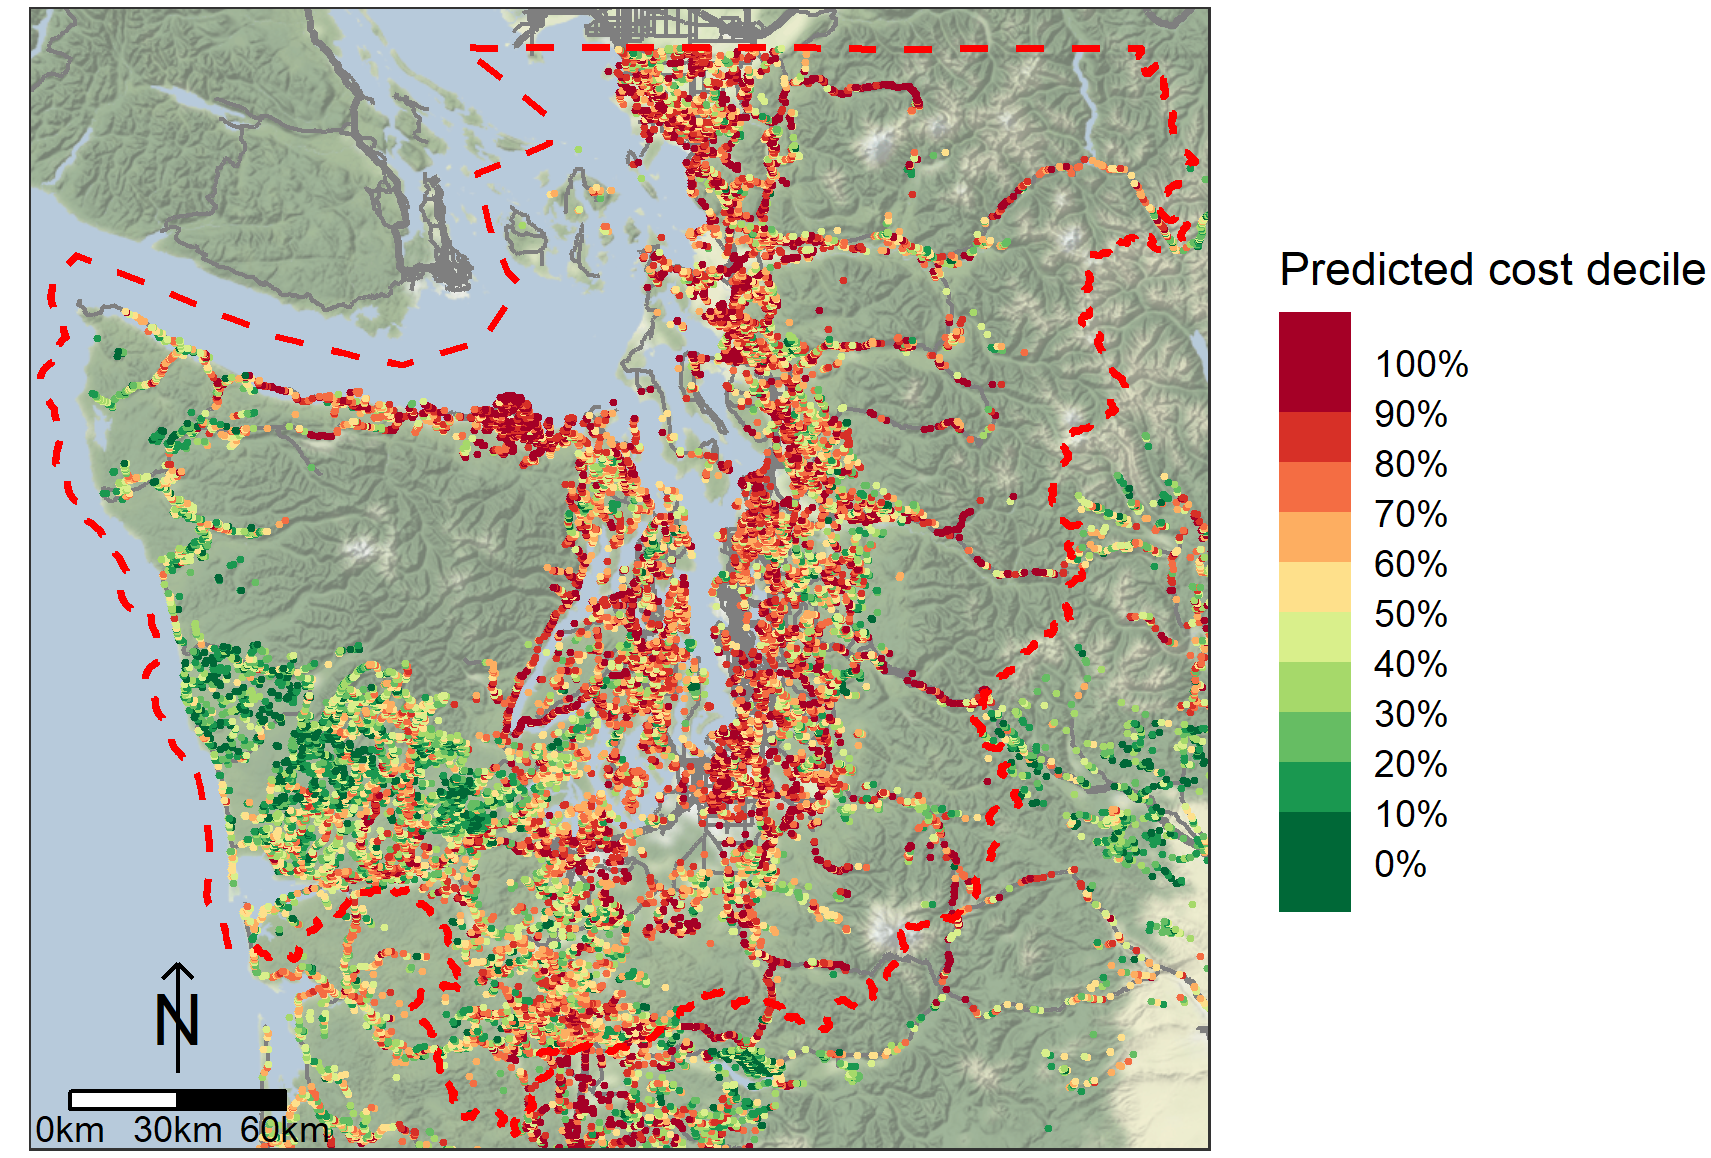
\includegraphics[width=10cm]{figures/predCost.png}
	\caption{Predicted cost percentiles for barrier culverts in the Case Area. Dashed red line indicates Case Area boundary.\label{fig:cost}}
\end{wrapfigure}%


Predictive cost models are currently being finalized by our research team. Figure~\ref{fig:cost} illustrates preliminary predicted cost percentiles using a fit from a boosted regression tree (BRT), one method under consideration. The BRT method builds an ensemble model of iterative regression trees fit on the residuals of earlier fits, systematically identifying variables useful for improving out-of-sample predictive power \citep{elith_working_2008}. In our team's ongoing work, we have found that such models can improve predictive accuracy (measured as training set root-mean square error) by 11\% over predictions from an ordinary least squares fit with variables selected by the analysts. 

For the proposed project, we will leverage the datasets and code we have already developed to explore the predictive performance of several parametric and non-parametric cost models, selecting the model that provides superior out-of-sample predictive power specifically in the Case Area. We will also seek out additional administrative data (i.e.\ project records) from state agencies and large private forestland owners to supplement the PNSHP with region-specific data. In doing so, we will provide consistent and granular barrier correction cost estimates that are applicable over the full Case Area. 

Importantly, our cost estimates will reflect inherent variability in correction costs between barriers. Accounting for heterogeneity in conservation/restoration costs often leads to efficiency gains, as a failure to do so implicitly assumes that all alternatives have the same costs \citep{babcock_targeting_1997}. For example, a recent study found that including cost information in a conservation planning tool increased habitat gains per dollar by as much as an order of magnitude \citep{field_quantifying_2019}. 

%Note that no previous studies in the fish passage optimization literature have used cost estimates based on statistical learning methods such as the BRT predictions demonstrated above. Instead, such studies most frequently rely on heuristic methods that assign barriers to a handful of cost categories (e.g.\ \cite{hermoso_accessible_2021}) or estimates during survey assessments conducted on far fewer barriers (e.g.\ \citep{ohanley_restoring_2013,king_toolkit_2017}), when costs are considered at all. 

\subsection*{Habitat model}

A primary objective in culvert barrier correction is increased access to quality salmon habitat. For each culvert restoration plan, defined as a combination of multiple culverts restored, we will quantify the expected increase in habitat quantity, measured as lineal distance, for the five species of Pacific salmon. Spatial dependence will drive restoration benefits, because the culvert restoration downstream determines the benefits from culvert restoration upstream. Estimated habitat quantity gains will be calculated using the USGS National Hydrography Dataset, NDHPlus High Resolution, and the WDFW FPDSI database, which contains information about fish species affected by culvert blockages. Our team has developed code to estimate similar lineal distance metrics for culvert restoration projects in the PNSHP database, which will be leveraged to estimate upstream habitat gained by correcting barriers within the Case Area cataloged in the FPDSI database. 

%The lineal distance measures will be supplemented with habitat quality metrics on a per species basis. Prioritization methods currently in use by barrier ownership entities often include some weighting metric for habitat quality. For example, a recent report assessing county-owned culverts in Clallam and Jefferson Counties uses intrinsic potential scores first developed by \cite{burnett_distribution_2007}, while the WDFW methodology assigns a fixed species-specific weight to habitat quantity based on an estimated number of adults potentially produced per habitat area \cite{noauthor_fish_2019}.
% Burnett, Kelly M., et al. "Distribution of salmon‐habitat potential relative to landscape characteristics and implications for conservation." Ecological Applications 17.1 (2007): 66-80.

In addition to habitat quantity (measured here as lineal distance), habitat quality plays an important role in the growth and survival of salmon \citep{Pess_2011}. The quality of salmon habitat is a function of many interacting attributes, including water temperature, instream flows, the presence of coarse woody debris, and the amount of fine sediment \citep{Bartz_2006,Isaak_2007}. All of these features of habitat quality are further affected by climatology, watershed geomorphology, and the connectivity of different habitat areas \citep{Caissie_2006, Rodeles_2019}, which means they may vary over time. For example, \citet{Battin_2007} found that future climate change and coordinated habitat restoration working together are likely to cause a shift in the distribution of salmon in Puget Sound as the quality of their habitat shifts around the landscape.

In a habitat restoration context, one of the key uncertainties is relating land use and land cover characteristics to the quality of salmon habitat \citep{Bartz_2006, Jorgensen_2009}. We will use statistical models to relate measures of salmon habitat quality to features of the environment sensu \citet{Bartz_2006} and \citet{Jorgensen_2009}. Specifically, our Research Scientist will work with co-PI Scheuerell to build upon these earlier efforts to develop a unitless metric of salmon habitat quality based on instream temperature and flow data, as well as upland features related to riparian forest density and composition, road density, elevation, and watershed area. In addition, we will consult with regional experts in salmon habitat restoration (e.g., Drs.\ George Pess and Tim Beechie, NOAA Fisheries) to ensure that we are capturing those features of the environment most likely to reflect the quality of salmon habitat.

\subsection*{Equity}

Equity is another important dimension to consider. In fact, \textcolor{red}{XXXX chose rank and score methods for barrier prioritization based on the need to ensure equity amongst tribal co-managers.} The concern was that a prioritization framework that simply maximizes expected salmon habitat given a budget constraint could potentially lead to a culvert restoration plan that only benefits a single user group. We will explore alternative equity strategies that prioritize restoration plans that provide an equitable distribution of habitat gains across user groups. While ideally we would explore solutions that achieve equity in allocating habitat gains across tribal usual and accustomed fishing areas, however, there is a lack of consensus around the usual and accustomed area boundaries. Thus, we will explore solutions that allocate habitat gains across alternative spatial units, e.g.\ watersheds and/or counties. We will also explore various equity metrics, e.g.\ a Gini coefficient, using geospatial data on all salmon runs in the injunction area together with geospatial data delineating watersheds in the Case Area. 

\subsection*{Risk mitigation}

Risk mitigation is yet another important factor to consider when selecting portfolios of barrier culverts to correct. Returns to investments in barrier culvert correction are risky, driven by the possibility of low salmon returns to habitat, population extinction driven by environmental shocks, and future human impacts including impacts to water quality through urbanization \citep{ettinger_prioritizing_2021}. 

%Additionally, climate change is expected to be a significant driver of returns to investments from barrier culvert correction. Climate change is projected to affect peak water flow during egg incubation, stream temperature during pre-spawning, and minimum flow during spawning \citep{battin_projected_2007}, with greatest impacts in high-elevation streams where barrier culverts are less common. Climate change may also affect channel bankfull width at road crossings, which in turn may cause a previously corrected culvert to revert to barrier status as the stream expands under future climate conditions. While expanded culvert designs can prevent this, they are often more expensive \cite{guillaume_mauger_climate_nodate}. Climate uncertainty will thus create risk of future culvert failure when smaller, cheaper correction designs are considered. 

Drawing from the literature on restoration portfolio diversification, we will estimate the degree to which the risk in returns to barrier culvert removal plans can be mitigated through diversification across salmon stocks. We will explore risk metrics ranging in complexity from a simple measure of the spread of investments across all salmon runs with habitat in the Case Area to more complex risk metrics that account for the probability negative impacts to salmon through urban growth. Geospatial data sources for salmon stocks and urban growth, respectively, include the \textcolor{red}{XXXX} and \href{https://geo.wa.gov/datasets/wa-geoservices::washington-state-city-urban-growth-areas/about}{Washington State City Urban Growth Areas}.


\subsection*{Optimization framework \label{sec:opt}}

There are several methods for defining cost-effective restoration plans that meet multiple planning goals (e.g.\ salmon habitat gains, equity considerations, and risk mitigation). We will explore alternative methods, selecting the approach that is most accessible and intuitive for our target users. One candidate method is the weighted objective function approach where managers specify importance weights for each of the objectives and the weighted sum of the objectives is maximized. Weights are constrained to the interval [0, 1] and sum to one, e.g.\ a manager solely interested in habitat would set the habitat importance weight to one and all other weights to zero. The problem will also include a budget constraint, such that expenditures on barrier restoration are less than or equal to a fixed budget $B$, and a hydrography constraint such that habitat gains from restoring any one barrier cannot be realized if there exist any downstream barriers to fish passage. 

In an alternative approach, one objective function is maximized and lower bounds are provided for all remaining objectives. For example, the problem can be defined to maximize habitat gains subject to each user group receiving some minimum fraction of the habitat gains or some minimum fraction of total expenditures, or a constraint such that habitat gains are distributed across some minimum number of salmon stocks. We will refer to this approach as the ``constraint-based'' method.

Finally, we will explore methods for identifying the Pareto Frontier, or the set of restoration plans for which no individual objective can be improved without making at least one objective worse off. Pareto Frontier analyses have been applied in the fish passage literature \citep[e.g.][]{couto_safeguarding_2021} and, by plotting restoration plans on the frontier along with interior solutions, the analysis allows managers to visually inspect tradeoffs between various objectives, which can make tradeoffs more transparent.

All problems will be solved using R, a free software environment that supports integer programming. A growing number of modern solvers are accessible through the R software environment, e.g.\ powerful solvers on the NEOS server can be accessed through the R Optimization Infrastructure or ROI package in R \citep{theussl2019roi}.

\subsection*{Research questions}

Our project will explore the following research questions:

\begin{enumerate}
\item \textbf{Environmental Conditions:} What environmental factors emerge from the literature as key drivers salmon habitat quality?
\item \textbf{Path Dependency:} Assuming that WSDOT addresses those barrier culverts blocking 90\% of habitat by 2030, what is the optimal restoration plan for all remaining barriers in the Washington Case Area? How does this compare with an optimal restoration plan that ignores the actions of WSDOT?
\item \textbf{Coordination:} What are the gains in benefits, e.g.\ habitat, equity, and risk avoidance, associated with coordination across actors (state agencies, local government, private landowners) and which of these multiple objectives is most affected by a lack of coordination across actors? 
\item \textbf{Tradeoffs:} Where in Washington injunction area (sub-basins/watersheds) are culvert restoration plans associated with trade-offs between potentially competing priorities (e.g., risk versus total habitat, equity versus total habitat), and where can ``win-wins'' occur (i.e., plans that meet multiple objectives without reducing others)? 
\item \textbf{Optimization versus Rank and Score:} What are the gains from optimization methods as compared to ``rank and score'' methods?
\item \textbf{Equity:} Is it possible to address equity issues in optimization methods for barrier culvert removal in Western Washington given a lack of agreement over boundaries of tribal usual and accustomed areas?
\end{enumerate}

\subsection*{Decision Support Tool (DST)}

To support the accessibility of our optimization framework for fish passage in Washington State, we will design and deploy an online user interface. While the central application DST is to determine restoration plans that maximize return on investment throughout the Case Area, given user preferences over multiple objectives and drawing from publicly-available datasets, we will also include several customizable features in the DST. For example, users will be able to input alternative culvert restoration plans to the DST to generate a report on how objectives (e.g. habitat miles, equity, and risk) compare between the user-selected restoration plan and the plan determined by our optimization framework. Users will also be able to select barrier owners (e.g.\ Kitsap county) and/or salmon species (e.g.\ Chinook) to focus the problem by excluding other owners/species. 

We will also explore enabling user data edits, e.g.\ user information on the existence of barrier culverts missing from the FPDSI database, similar to the ``Wild West'' option in FishWerks, and user information on barrier culverts on private lands where the landowner is unwilling to engage in fish passage restoration. Further options for user-provided data will be discussed and determined in workshops with key user groups (see Engagement and Communication Plan).

Defining gains to objectives (e.g.\ habitat) consistently across all barrier culverts in the Case Area allows for comparison and coordinated restoration planning. However, we also strive to support existing efforts by cities and counties in Washington who are working on constructing prioritization indices tailored for their own specific needs. Through cataloging the methods and datasets for fish passage prioritization indices for all relevant entities in Washington, we will explore the possibility of including adopted prioritization indices in our optimization framework. In order to include these indices, we would modify the indices to remove any components of the index related to restoration costs or upstream/downstream configuration as our framework explicitly accounts for these culvert characteristics. Users could select the modified prioritization index of interest to them (e.g. the modified prioritization index from King County) and use the tool to determine the culvert restoration package in King County that maximizes the modified prioritization index (from the perspective of King County) subject to a budget constraint and the hydrography of the system.

Finally, we will incorporate a number of scenario-planning tools based on needs identified by key user groups (See Engagement and Communication Plan). These features will allow users to explore how plans identified by the optimization tool vary based on alternative futures determined by factors external to the decision-maker. For example, given that WSDOT is mandated to correct enough barriers to open 90\% blocked habitat by 2030, counties and other entities may want to consider scenarios where all state-owned culverts have been fixed, or alternative subsets that represent the 90\% habitat target. In doing so, users can better capitalize on the massive infrastructure investments WSDOT is expected to make in order to comply with the injunction. We will also consider, as a starting point, climate and urbanization scenarios, two factors which are likely to affect both the value and costs of specific barrier correction actions.
  
The online app created with the Shiny package for R and hosted on the Shiny Server. Similar tools have been built using various proprietary software programs \citep{ohanley_optipass_2015, moody_pet_2017}. Through using an open-source optimization framework coupled with an open-source user interface we maximize accessibility and customizability. 


\section{Project Evaluation}

Our project objectives can be grouped into three broad categories that will be evaluated independently as described here. 

First, a primary objective of the project is to utilize our framework to explore critical research questions related to the science and economics of barrier culvert removal in Washington State. Specifically, we will characterize the tradeoffs associated with barrier culvert replacement, evaluate the performance of PI methods, which are widely used throughout the Washington Case Area, and estimate gains from coordination across barrier culvert owners in Washington (e.g.\ additional habitat realized when the state works in coordination with counties). These questions will be explored in journal publications, which will be evaluated according to the quality of the journal, popular press coverage of the publications, and standard citation metrics.


A second primary objective primary objective of the project is to produce a DST that can inform decisions regarding fish passage projects in Washington State.  We will evaluate the effectiveness of these efforts through evaluating workshop attendance and post-workshop surveys collected in Workshops 1 and 3 (see Engagement and Communication Plan), and through analytics collected through the R Shiny application (e.g.\ the number of unique users, length of use, user location, etc.).

We also seek to use the project to train junior scientists to produce research that is actionable, publishable, and reproducible. We will evaluate these efforts based on both inputs and outputs. Inputs to student training are the opportunities that the PIs offer students (e.g.\ to speak at meetings, present results, join meetings, attend conferences) and approaches to engaging students. Outputs are the quality of student work, the quality of the questions and concerns raised by students as related to the research project, and the student engagement in the project (e.g.\ is the student excited to attend workshops with managers, tribes, and other stakeholders). 

\section{Timeline}
\begin{table}[htb]
\small
\begin{tabular}{|p{0.275\linewidth} | p{0.08\linewidth} | p{0.08\linewidth} | p{0.08\linewidth} | p{0.08\linewidth} | p{0.08\linewidth} | p{0.08\linewidth} | p{0.08\linewidth} |}\hline
 &  Oct/Dec &  Jan/Mar  & Apr/Jun & Jul/Sept  & Oct/Dec & Jan/Mar & Apr/Jun \\
 &  Q1 &  Q2  & Q3 & Q4  & Q5 & Q6 & Q7\\\hline
Workshop 1: Gathering Input & \cellcolor{gray!50}  &   &  & &   &  & \\ \hline
Catalog prioritization indices &  \cellcolor{gray!50}  &  \cellcolor{gray!50}  &  & &   &  & \\\hline
Generate salmon habitat quantity dataset building off existing work products & \cellcolor{gray!50}  &  \cellcolor{gray!50}  & \cellcolor{gray!50}  & &   &  & \\\hline
Generate barrier removal cost estimates building off existing work products &  \cellcolor{gray!50} & \cellcolor{gray!50}   & \cellcolor{gray!50}  & \cellcolor{gray!50} &   &  & \\\hline
Generate habitat quality dataset &  \cellcolor{gray!50} &   \cellcolor{gray!50} &  \cellcolor{gray!50} & \cellcolor{gray!50} &   &  & \\\hline
Generate equity metrics and data & \cellcolor{gray!50}  &   \cellcolor{gray!50} & \cellcolor{gray!50}  & \cellcolor{gray!50} &   &  & \\\hline
Generate risk mitigation metrics and data & \cellcolor{gray!50}  &  \cellcolor{gray!50}  &\cellcolor{gray!50}   &\cellcolor{gray!50}  &   &  & \\\hline
Develop optimization code building off existing template code & \cellcolor{gray!50}  & \cellcolor{gray!50}   & \cellcolor{gray!50}  &\cellcolor{gray!50}  &  &   & \\\hline
%Develop code to analyze the optimization results building off existing work products and template code & \cellcolor{gray!50}  &  \cellcolor{gray!50}  & \cellcolor{gray!50}  & \cellcolor{gray!50} &   &  & \\\hline
Analyze optimal solutions &  &   & \cellcolor{gray!50}  & \cellcolor{gray!50} &  \cellcolor{gray!50}  & \cellcolor{gray!50}  & \\\hline
Workshop 2: Soliciting Feedback &  &   &  & \cellcolor{gray!50} &   &  & \\\hline
Integrate feedback from Workshop 2 &  &   &  & &  \cellcolor{gray!50}  &  \cellcolor{gray!50} & \cellcolor{gray!50} \\\hline
Develop the R Shiny app &  &   &  &  \cellcolor{gray!50} &  \cellcolor{gray!50}  &  \cellcolor{gray!50} & \cellcolor{gray!50} \\\hline
Prepare manuscripts for publication &  &   &  & &   &  \cellcolor{gray!50} & \cellcolor{gray!50} \\\hline
Workshop 3: DST Demonstration and Launch &  &   &  & &   &  & \cellcolor{gray!50} \\\hline

\end{tabular}
\end{table}
\FloatBarrier
 